\section{Appendix}

Here, we provide a detailed architectural analysis of existing agent RL infrastructures, accompanied by illustrative diagrams.

\begin{figure}[h]
  \centering
  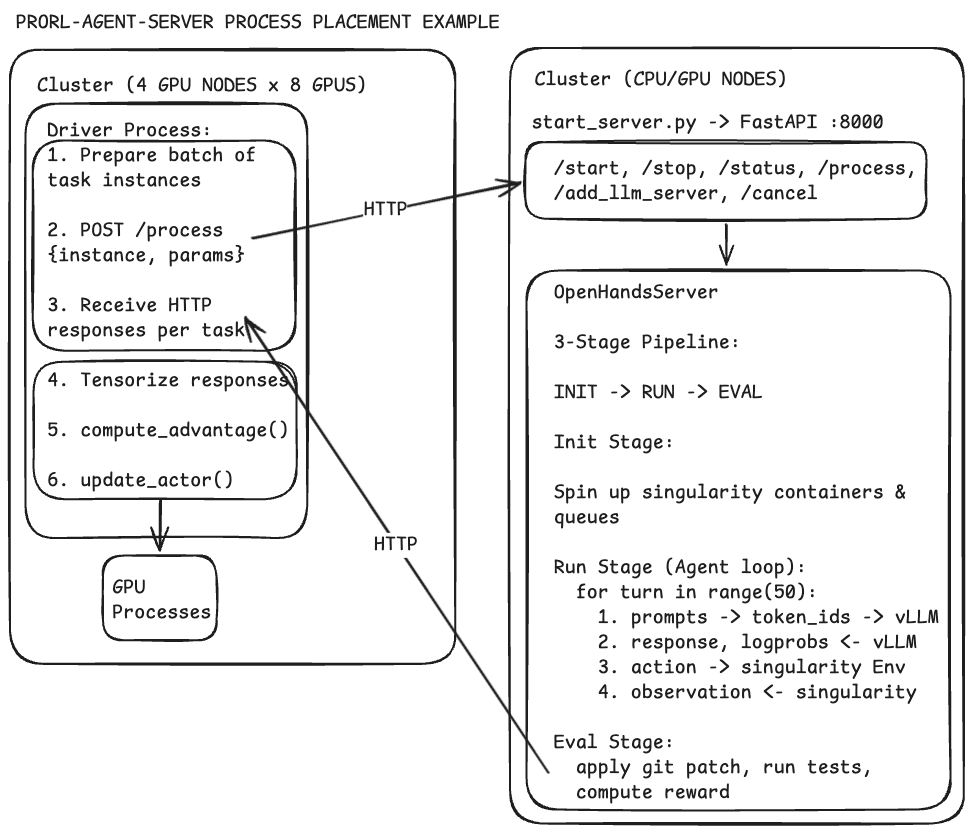
\includegraphics[width=0.9\linewidth]{figures/prorl_agent.png}
  \caption{\prorlagent separates the full agentic rollout lifecycle, spanning environment management to reward computation, from GPU-intensive training, thereby decoupling I/O-intensive rollout from training.}
  \label{fig:prorl_agent}
\end{figure}

\begin{figure}[h]
  \centering
  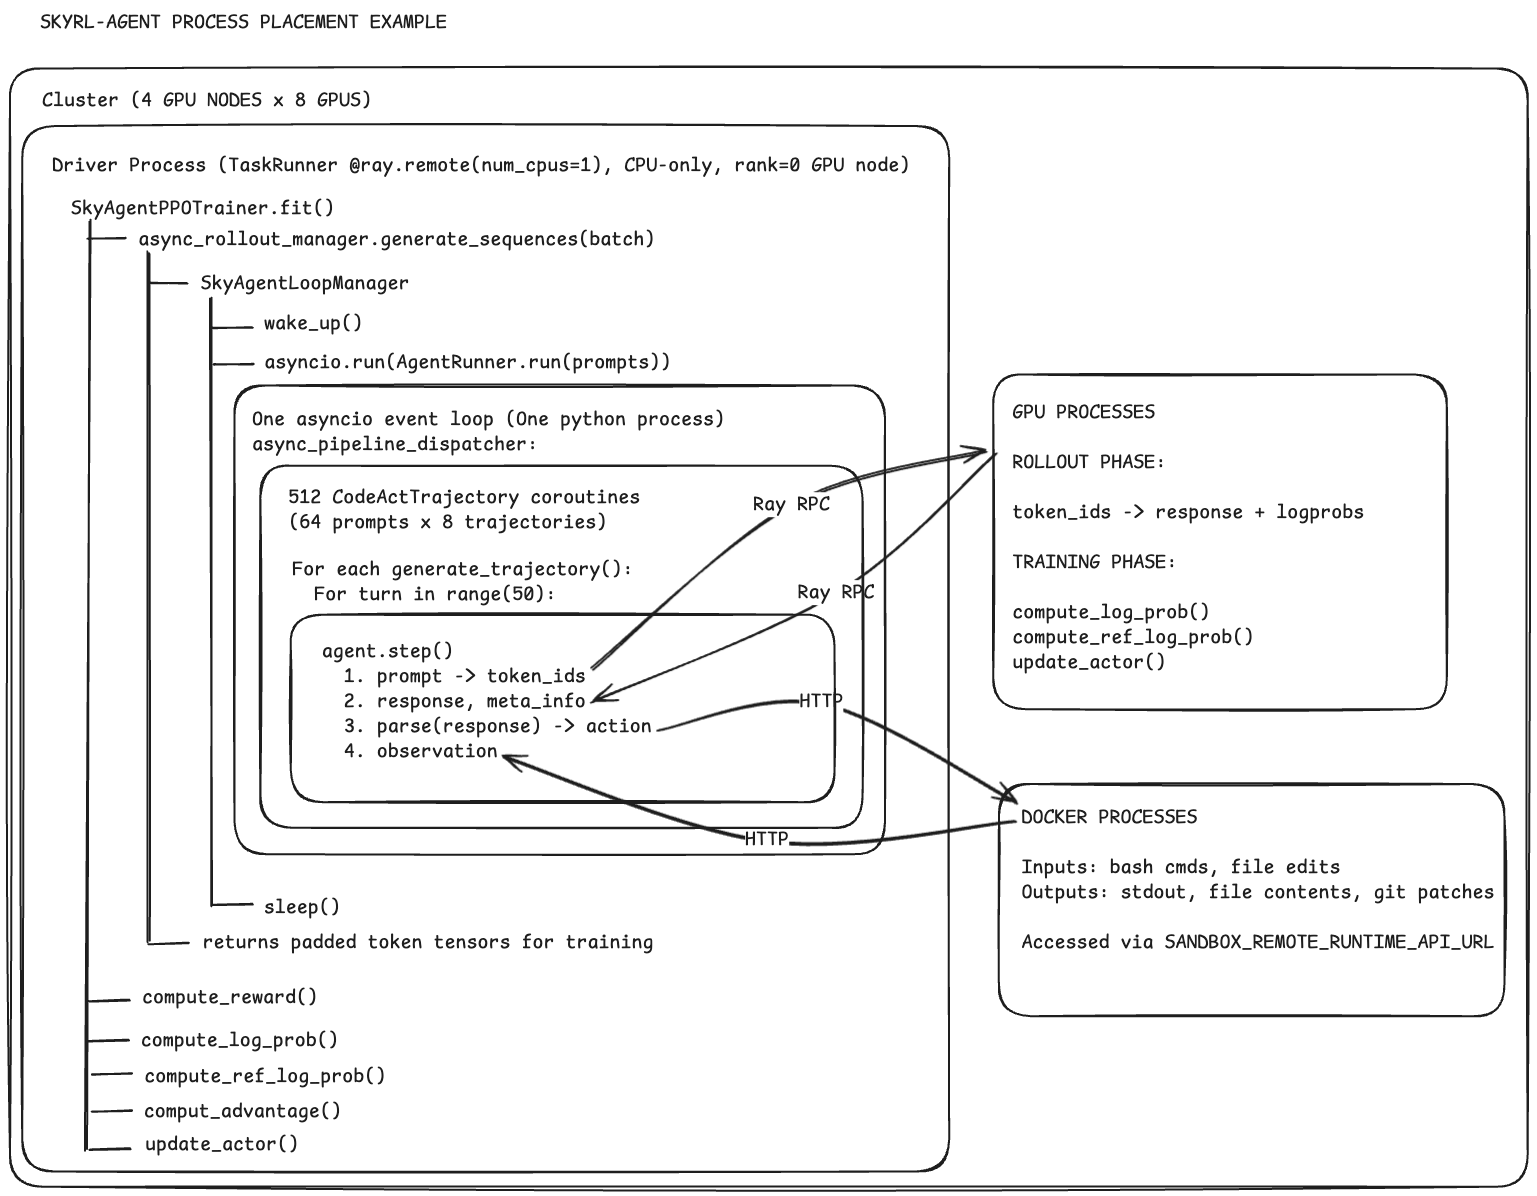
\includegraphics[width=1\linewidth]{figures/sky_rl_agent.png}
\caption{
\textbf{SkyRL-Agent.} The training driver runs concurrent trajectory-generation coroutines on a single CPU process. It controls the multi-turn agent loop, queries a remote vLLM server for inference, and interacts with remote environment containers for execution. Although inference and environment execution are offloaded, rollout control remains inside the training driver.}
  \label{fig:skyrl_agent}
\end{figure}

\begin{figure}[h]
  \centering
  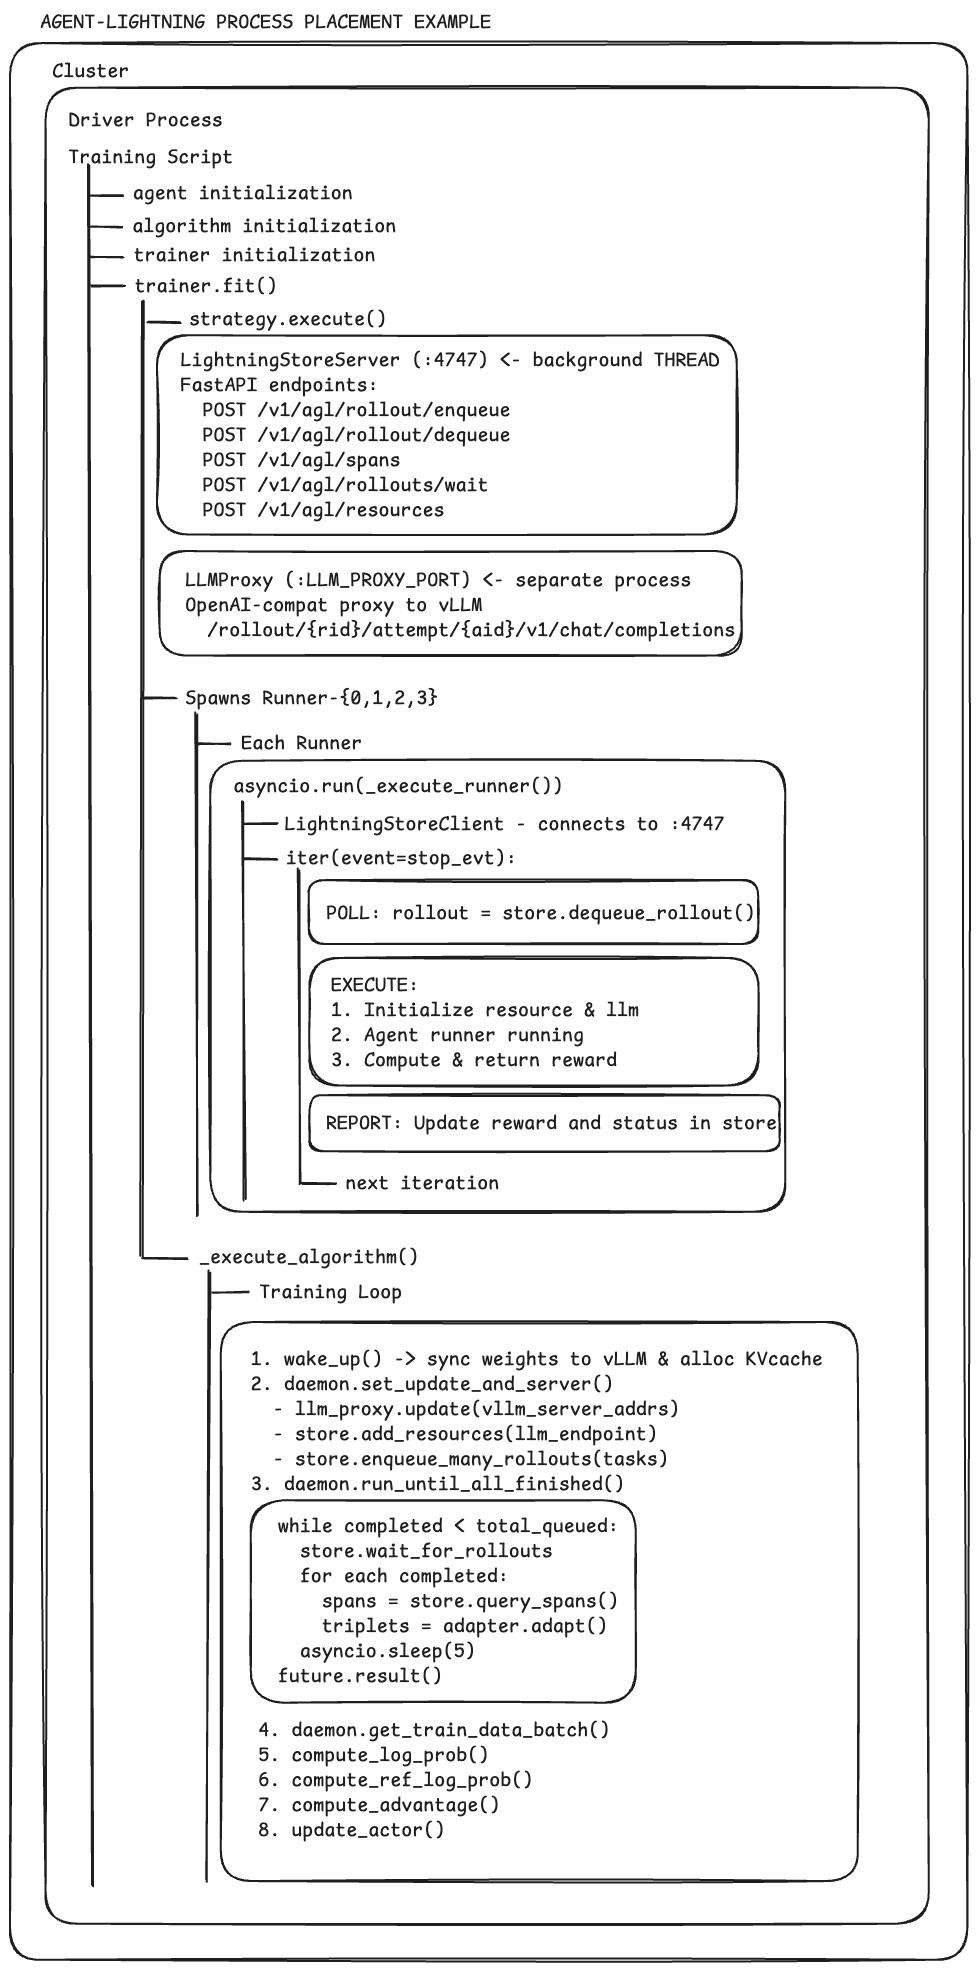
\includegraphics[width=0.55\textwidth]{figures/agent_lightning.png}
\caption{\textbf{Agent Lightning.} Agent Lightning places the training loop, the \texttt{LightningStoreServer}, and all rollout workers within a single process tree. The store runs as a background thread, while rollout workers are spawned as child processes from the trainer. As a result, rollout does not have an independent service lifecycle: if the training process terminates, the store also stops and the rollout workers are disrupted. Thus, rollout remains managed within the training stack rather than being cleanly decoupled.}
  \label{fig:agent_lightning}
\end{figure}


\begin{figure}[h]
  \centering
  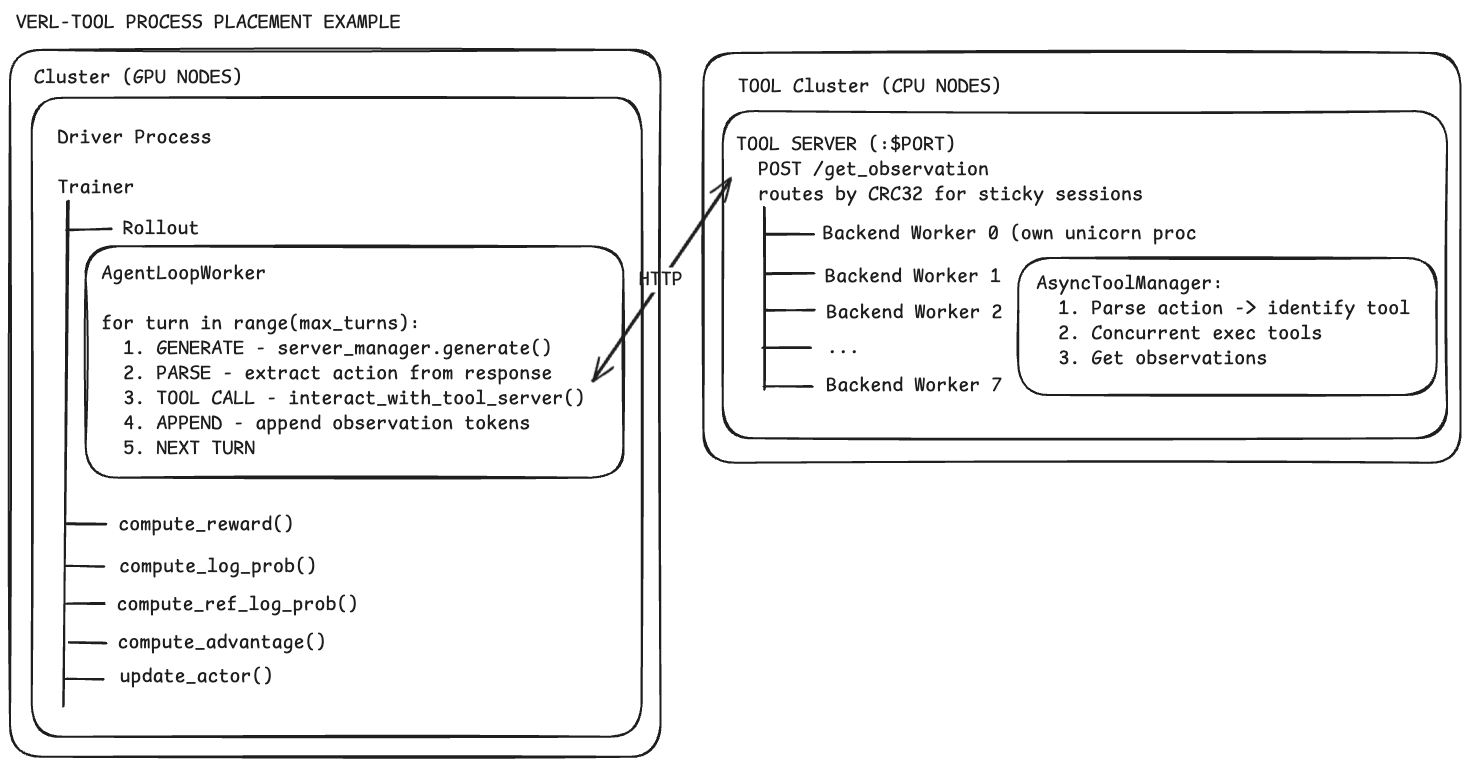
\includegraphics[width=1\textwidth]{figures/verl_tool.png}
\caption{\textbf{VeRL-Tool.} VeRL-Tool extends the standard veRL trainer to support multi-turn agent rollouts. The training system manages the agent loop and trajectory collection, while tool execution is offloaded to a separate CPU-based environment service. In this design, rollout control remains inside the trainer.}
  \label{fig:verl_tool}
\end{figure}

\begin{figure}[h]
  \centering
  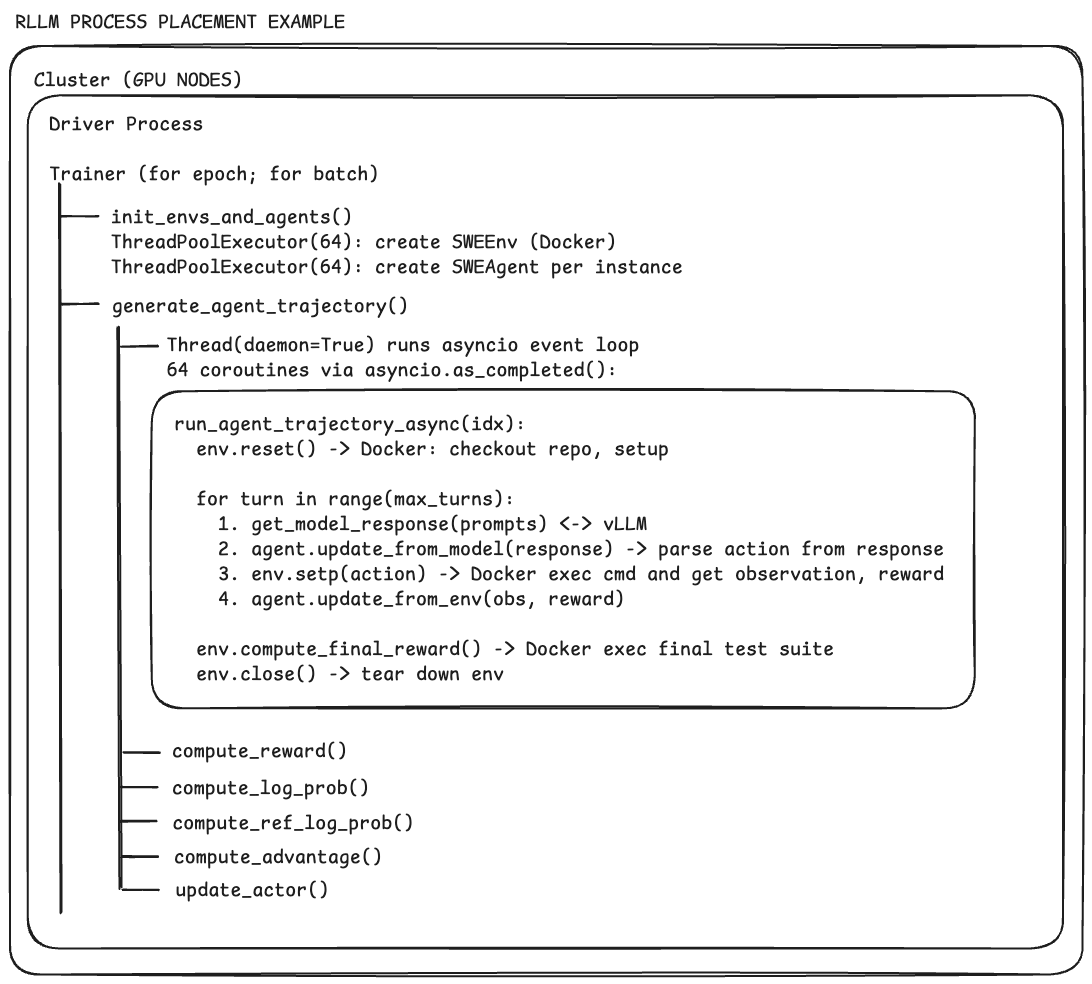
\includegraphics[width=0.7\textwidth]{figures/rllm.png}
\caption{\textbf{rLLM: rollout embedded in a monolithic training driver.} rLLM is built on a heavily modified fork of veRL. The agent loop, environment management, and trajectory orchestration all reside within a single driver process. There is no independent rollout service, no persistent trajectory buffer, and no possibility of the rollout surviving independently of the training driver. The full rollout lifecycle remains tightly coupled with the training stack.}
  \label{fig:rllm}
\end{figure}

\begin{figure}[h]
  \centering
  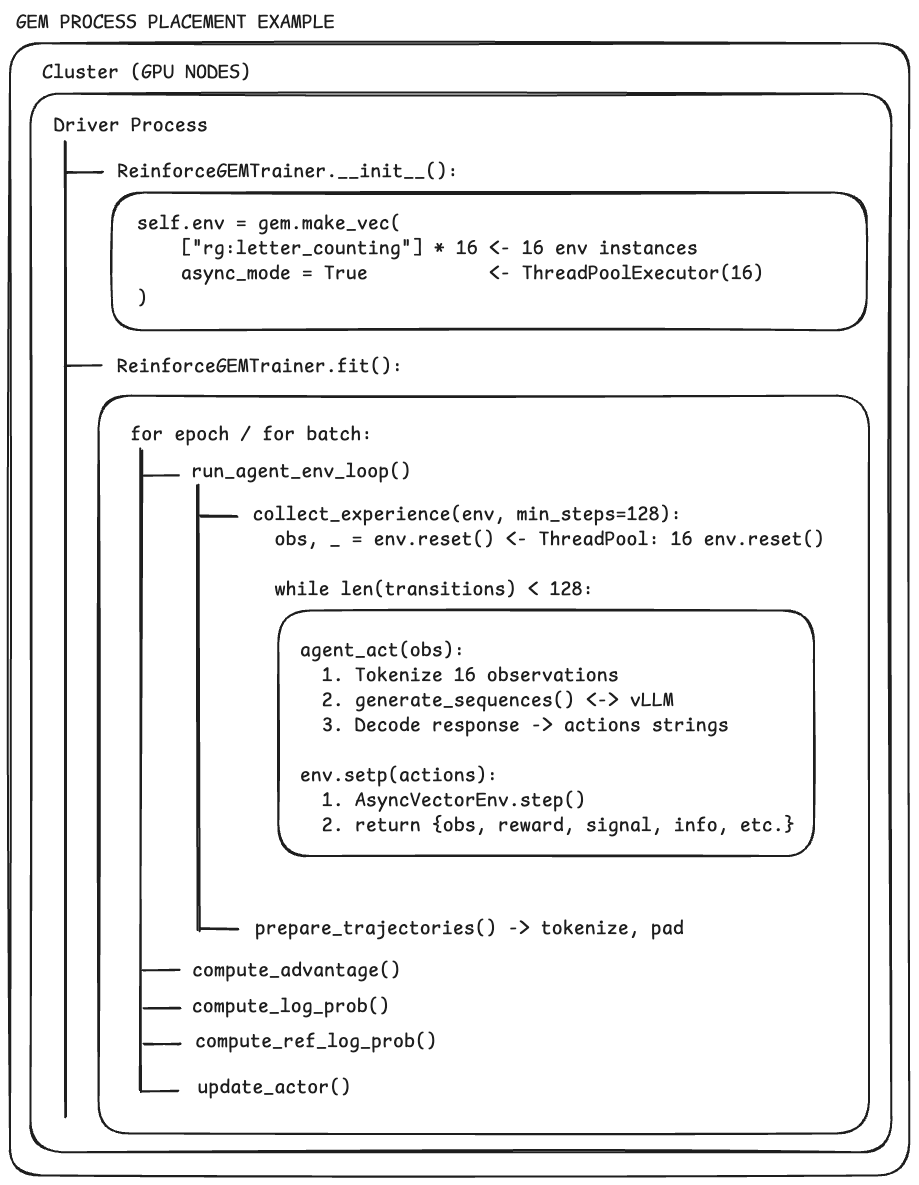
\includegraphics[width=0.7\textwidth]{figures/gem.png}
\caption{\textbf{GEM.} GEM keeps environment execution inside the training process. Environments are instantiated as in-memory Python objects, and environment stepping is performed through direct \texttt{env.step()} calls, with parallelism provided only by \texttt{ThreadPoolExecutor} threads in the same address space. A single driver process orchestrates both rollout and training, while GPU workers are accessed remotely via Ray RPC. As a result, the environment and rollout lifecycle remain fully embedded in the training stack.}
  \label{fig:gem}
\end{figure}